\documentclass[11pt]{article}
\usepackage{float}
\usepackage{tikz}
\usetikzlibrary{automata, positioning}
% NOTE: Add in the relevant information to the commands below; or, if you'll be using the same information frequently, add these commands at the top of paolo-pset.tex file. 
\newcommand{\name}{Agustín Esteva}
\newcommand{\email}{aesteva@uchicago.edu}
\newcommand{\classnum}{23500}
\newcommand{\subject}{Markov Chains, Martingales, and Brownian Motion}
\newcommand{\instructors}{Stephen Yearwood}
\newcommand{\assignment}{Problem Set 2}
\newcommand{\semester}{Spring 2025}
\newcommand{\duedate}{04/11/2025}
\newcommand{\bA}{\mathbf{A}}
\newcommand{\bB}{\mathbf{B}}
\newcommand{\bC}{\mathbf{C}}
\newcommand{\bD}{\mathbf{D}}
\newcommand{\bE}{\mathbf{E}}
\newcommand{\bF}{\mathbf{F}}
\newcommand{\bG}{\mathbf{G}}
\newcommand{\bH}{\mathbf{H}}
\newcommand{\bI}{\mathbf{I}}
\newcommand{\bJ}{\mathbf{J}}
\newcommand{\bK}{\mathbf{K}}
\newcommand{\bL}{\mathbf{L}}
\newcommand{\bM}{\mathbf{M}}
\newcommand{\bN}{\mathbf{N}}
\newcommand{\bO}{\mathbf{O}}
\newcommand{\bP}{\mathbf{P}}
\newcommand{\bQ}{\mathbf{Q}}
\newcommand{\bR}{\mathbf{R}}
\newcommand{\bS}{\mathbf{S}}
\newcommand{\bT}{\mathbf{T}}
\newcommand{\bU}{\mathbf{U}}
\newcommand{\bV}{\mathbf{V}}
\newcommand{\bW}{\mathbf{W}}
\newcommand{\bX}{\mathbf{X}}
\newcommand{\bY}{\mathbf{Y}}
\newcommand{\bZ}{\mathbf{Z}}
\newcommand{\Vol}{\text{Vol}}

%% blackboard bold math capitals
\newcommand{\bbA}{\mathbb{A}}
\newcommand{\bbB}{\mathbb{B}}
\newcommand{\bbC}{\mathbb{C}}
\newcommand{\bbD}{\mathbb{D}}
\newcommand{\bbE}{\mathbb{E}}
\newcommand{\bbF}{\mathbb{F}}
\newcommand{\bbG}{\mathbb{G}}
\newcommand{\bbH}{\mathbb{H}}
\newcommand{\bbI}{\mathbb{I}}
\newcommand{\bbJ}{\mathbb{J}}
\newcommand{\bbK}{\mathbb{K}}
\newcommand{\bbL}{\mathbb{L}}
\newcommand{\bbM}{\mathbb{M}}
\newcommand{\bbN}{\mathbb{N}}
\newcommand{\bbO}{\mathbb{O}}
\newcommand{\bbP}{\mathbb{P}}
\newcommand{\bbQ}{\mathbb{Q}}
\newcommand{\bbR}{\mathbb{R}}
\newcommand{\bbS}{\mathbb{S}}
\newcommand{\bbT}{\mathbb{T}}
\newcommand{\bbU}{\mathbb{U}}
\newcommand{\bbV}{\mathbb{V}}
\newcommand{\bbW}{\mathbb{W}}
\newcommand{\bbX}{\mathbb{X}}
\newcommand{\bbY}{\mathbb{Y}}
\newcommand{\bbZ}{\mathbb{Z}}

%% script math capitals
\newcommand{\sA}{\mathscr{A}}
\newcommand{\sB}{\mathscr{B}}
\newcommand{\sC}{\mathscr{C}}
\newcommand{\sD}{\mathscr{D}}
\newcommand{\sE}{\mathscr{E}}
\newcommand{\sF}{\mathscr{F}}
\newcommand{\sG}{\mathscr{G}}
\newcommand{\sH}{\mathscr{H}}
\newcommand{\sI}{\mathscr{I}}
\newcommand{\sJ}{\mathscr{J}}
\newcommand{\sK}{\mathscr{K}}
\newcommand{\sL}{\mathscr{L}}
\newcommand{\sM}{\mathscr{M}}
\newcommand{\sN}{\mathscr{N}}
\newcommand{\sO}{\mathscr{O}}
\newcommand{\sP}{\mathscr{P}}
\newcommand{\sQ}{\mathscr{Q}}
\newcommand{\sR}{\mathscr{R}}
\newcommand{\sS}{\mathscr{S}}
\newcommand{\sT}{\mathscr{T}}
\newcommand{\sU}{\mathscr{U}}
\newcommand{\sV}{\mathscr{V}}
\newcommand{\sW}{\mathscr{W}}
\newcommand{\sX}{\mathscr{X}}
\newcommand{\sY}{\mathscr{Y}}
\newcommand{\sZ}{\mathscr{Z}}


\renewcommand{\emptyset}{\O}

\newcommand{\abs}[1]{\lvert #1 \rvert}
\newcommand{\norm}[1]{\lVert #1 \rVert}
\newcommand{\sm}{\setminus}


\newcommand{\sarr}{\rightarrow}
\newcommand{\arr}{\longrightarrow}

% NOTE: Defining collaborators is optional; to not list collaborators, comment out the line below.
%\newcommand{\collaborators}{Alyssa P. Hacker (\texttt{aphacker}), Ben Bitdiddle (\texttt{bitdiddle})}

% Copyright 2021 Paolo Adajar (padajar.com, paoloadajar@mit.edu)
% 
% Permission is hereby granted, free of charge, to any person obtaining a copy of this software and associated documentation files (the "Software"), to deal in the Software without restriction, including without limitation the rights to use, copy, modify, merge, publish, distribute, sublicense, and/or sell copies of the Software, and to permit persons to whom the Software is furnished to do so, subject to the following conditions:
%
% The above copyright notice and this permission notice shall be included in all copies or substantial portions of the Software.
% 
% THE SOFTWARE IS PROVIDED "AS IS", WITHOUT WARRANTY OF ANY KIND, EXPRESS OR IMPLIED, INCLUDING BUT NOT LIMITED TO THE WARRANTIES OF MERCHANTABILITY, FITNESS FOR A PARTICULAR PURPOSE AND NONINFRINGEMENT. IN NO EVENT SHALL THE AUTHORS OR COPYRIGHT HOLDERS BE LIABLE FOR ANY CLAIM, DAMAGES OR OTHER LIABILITY, WHETHER IN AN ACTION OF CONTRACT, TORT OR OTHERWISE, ARISING FROM, OUT OF OR IN CONNECTION WITH THE SOFTWARE OR THE USE OR OTHER DEALINGS IN THE SOFTWARE.

\usepackage{fullpage}
\usepackage{enumitem}
\usepackage{amsfonts, amssymb, amsmath,amsthm}
\usepackage{mathtools}
\usepackage[pdftex, pdfauthor={\name}, pdftitle={\classnum~\assignment}]{hyperref}
\usepackage[dvipsnames]{xcolor}
\usepackage{bbm}
\usepackage{graphicx}
\usepackage{mathrsfs}
\usepackage{pdfpages}
\usepackage{tabularx}
\usepackage{pdflscape}
\usepackage{makecell}
\usepackage{booktabs}
\usepackage{natbib}
\usepackage{caption}
\usepackage{subcaption}
\usepackage{physics}
\usepackage[many]{tcolorbox}
\usepackage{version}
\usepackage{ifthen}
\usepackage{cancel}
\usepackage{listings}
\usepackage{courier}

\usepackage{tikz}
\usepackage{istgame}

\hypersetup{
	colorlinks=true,
	linkcolor=blue,
	filecolor=magenta,
	urlcolor=blue,
}

\setlength{\parindent}{0mm}
\setlength{\parskip}{2mm}

\setlist[enumerate]{label=({\alph*})}
\setlist[enumerate, 2]{label=({\roman*})}

\allowdisplaybreaks[1]

\newcommand{\psetheader}{
	\ifthenelse{\isundefined{\collaborators}}{
		\begin{center}
			{\setlength{\parindent}{0cm} \setlength{\parskip}{0mm}
				
				{\textbf{\classnum~\semester:~\assignment} \hfill \name}
				
				\subject \hfill \href{mailto:\email}{\tt \email}
				
				Instructor(s):~\instructors \hfill Due Date:~\duedate	
				
				\hrulefill}
		\end{center}
	}{
		\begin{center}
			{\setlength{\parindent}{0cm} \setlength{\parskip}{0mm}
				
				{\textbf{\classnum~\semester:~\assignment} \hfill \name\footnote{Collaborator(s): \collaborators}}
				
				\subject \hfill \href{mailto:\email}{\tt \email}
				
				Instructor(s):~\instructors \hfill Due Date:~\duedate	
				
				\hrulefill}
		\end{center}
	}
}

\renewcommand{\thepage}{\classnum~\assignment \hfill \arabic{page}}

\makeatletter
\def\points{\@ifnextchar[{\@with}{\@without}}
\def\@with[#1]#2{{\ifthenelse{\equal{#2}{1}}{{[1 point, #1]}}{{[#2 points, #1]}}}}
\def\@without#1{\ifthenelse{\equal{#1}{1}}{{[1 point]}}{{[#1 points]}}}
\makeatother

\newtheoremstyle{theorem-custom}%
{}{}%
{}{}%
{\itshape}{.}%
{ }%
{\thmname{#1}\thmnumber{ #2}\thmnote{ (#3)}}

\theoremstyle{theorem-custom}

\newtheorem{theorem}{Theorem}
\newtheorem{lemma}[theorem]{Lemma}
\newtheorem{example}[theorem]{Example}

\newenvironment{problem}[1]{\color{black} #1}{}

\newenvironment{solution}{%
	\leavevmode\begin{tcolorbox}[breakable, colback=green!5!white,colframe=green!75!black, enhanced jigsaw] \proof[\scshape Solution:] \setlength{\parskip}{2mm}%
	}{\renewcommand{\qedsymbol}{$\blacksquare$} \endproof \end{tcolorbox}}

\newenvironment{reflection}{\begin{tcolorbox}[breakable, colback=black!8!white,colframe=black!60!white, enhanced jigsaw, parbox = false]\textsc{Reflections:}}{\end{tcolorbox}}

\newcommand{\qedh}{\renewcommand{\qedsymbol}{$\blacksquare$}\qedhere}

\definecolor{mygreen}{rgb}{0,0.6,0}
\definecolor{mygray}{rgb}{0.5,0.5,0.5}
\definecolor{mymauve}{rgb}{0.58,0,0.82}

% from https://github.com/satejsoman/stata-lstlisting
% language definition
\lstdefinelanguage{Stata}{
	% System commands
	morekeywords=[1]{regress, reg, summarize, sum, display, di, generate, gen, bysort, use, import, delimited, predict, quietly, probit, margins, test},
	% Reserved words
	morekeywords=[2]{aggregate, array, boolean, break, byte, case, catch, class, colvector, complex, const, continue, default, delegate, delete, do, double, else, eltypedef, end, enum, explicit, export, external, float, for, friend, function, global, goto, if, inline, int, local, long, mata, matrix, namespace, new, numeric, NULL, operator, orgtypedef, pointer, polymorphic, pragma, private, protected, public, quad, real, return, rowvector, scalar, short, signed, static, strL, string, struct, super, switch, template, this, throw, transmorphic, try, typedef, typename, union, unsigned, using, vector, version, virtual, void, volatile, while,},
	% Keywords
	morekeywords=[3]{forvalues, foreach, set},
	% Date and time functions
	morekeywords=[4]{bofd, Cdhms, Chms, Clock, clock, Cmdyhms, Cofc, cofC, Cofd, cofd, daily, date, day, dhms, dofb, dofC, dofc, dofh, dofm, dofq, dofw, dofy, dow, doy, halfyear, halfyearly, hh, hhC, hms, hofd, hours, mdy, mdyhms, minutes, mm, mmC, mofd, month, monthly, msofhours, msofminutes, msofseconds, qofd, quarter, quarterly, seconds, ss, ssC, tC, tc, td, th, tm, tq, tw, week, weekly, wofd, year, yearly, yh, ym, yofd, yq, yw,},
	% Mathematical functions
	morekeywords=[5]{abs, ceil, cloglog, comb, digamma, exp, expm1, floor, int, invcloglog, invlogit, ln, ln1m, ln, ln1p, ln, lnfactorial, lngamma, log, log10, log1m, log1p, logit, max, min, mod, reldif, round, sign, sqrt, sum, trigamma, trunc,},
	% Matrix functions
	morekeywords=[6]{cholesky, coleqnumb, colnfreeparms, colnumb, colsof, corr, det, diag, diag0cnt, el, get, hadamard, I, inv, invsym, issymmetric, J, matmissing, matuniform, mreldif, nullmat, roweqnumb, rownfreeparms, rownumb, rowsof, sweep, trace, vec, vecdiag, },
	% Programming functions
	morekeywords=[7]{autocode, byteorder, c, _caller, chop, abs, clip, cond, e, fileexists, fileread, filereaderror, filewrite, float, fmtwidth, has_eprop, inlist, inrange, irecode, matrix, maxbyte, maxdouble, maxfloat, maxint, maxlong, mi, minbyte, mindouble, minfloat, minint, minlong, missing, r, recode, replay, return, s, scalar, smallestdouble,},
	% Random-number functions
	morekeywords=[8]{rbeta, rbinomial, rcauchy, rchi2, rexponential, rgamma, rhypergeometric, rigaussian, rlaplace, rlogistic, rnbinomial, rnormal, rpoisson, rt, runiform, runiformint, rweibull, rweibullph,},
	% Selecting time-span functions
	morekeywords=[9]{tin, twithin,},
	% Statistical functions
	morekeywords=[10]{betaden, binomial, binomialp, binomialtail, binormal, cauchy, cauchyden, cauchytail, chi2, chi2den, chi2tail, dgammapda, dgammapdada, dgammapdadx, dgammapdx, dgammapdxdx, dunnettprob, exponential, exponentialden, exponentialtail, F, Fden, Ftail, gammaden, gammap, gammaptail, hypergeometric, hypergeometricp, ibeta, ibetatail, igaussian, igaussianden, igaussiantail, invbinomial, invbinomialtail, invcauchy, invcauchytail, invchi2, invchi2tail, invdunnettprob, invexponential, invexponentialtail, invF, invFtail, invgammap, invgammaptail, invibeta, invibetatail, invigaussian, invigaussiantail, invlaplace, invlaplacetail, invlogistic, invlogistictail, invnbinomial, invnbinomialtail, invnchi2, invnF, invnFtail, invnibeta, invnormal, invnt, invnttail, invpoisson, invpoissontail, invt, invttail, invtukeyprob, invweibull, invweibullph, invweibullphtail, invweibulltail, laplace, laplaceden, laplacetail, lncauchyden, lnigammaden, lnigaussianden, lniwishartden, lnlaplaceden, lnmvnormalden, lnnormal, lnnormalden, lnwishartden, logistic, logisticden, logistictail, nbetaden, nbinomial, nbinomialp, nbinomialtail, nchi2, nchi2den, nchi2tail, nF, nFden, nFtail, nibeta, normal, normalden, npnchi2, npnF, npnt, nt, ntden, nttail, poisson, poissonp, poissontail, t, tden, ttail, tukeyprob, weibull, weibullden, weibullph, weibullphden, weibullphtail, weibulltail,},
	% String functions 
	morekeywords=[11]{abbrev, char, collatorlocale, collatorversion, indexnot, plural, plural, real, regexm, regexr, regexs, soundex, soundex_nara, strcat, strdup, string, strofreal, string, strofreal, stritrim, strlen, strlower, strltrim, strmatch, strofreal, strofreal, strpos, strproper, strreverse, strrpos, strrtrim, strtoname, strtrim, strupper, subinstr, subinword, substr, tobytes, uchar, udstrlen, udsubstr, uisdigit, uisletter, ustrcompare, ustrcompareex, ustrfix, ustrfrom, ustrinvalidcnt, ustrleft, ustrlen, ustrlower, ustrltrim, ustrnormalize, ustrpos, ustrregexm, ustrregexra, ustrregexrf, ustrregexs, ustrreverse, ustrright, ustrrpos, ustrrtrim, ustrsortkey, ustrsortkeyex, ustrtitle, ustrto, ustrtohex, ustrtoname, ustrtrim, ustrunescape, ustrupper, ustrword, ustrwordcount, usubinstr, usubstr, word, wordbreaklocale, worcount,},
	% Trig functions
	morekeywords=[12]{acos, acosh, asin, asinh, atan, atanh, cos, cosh, sin, sinh, tan, tanh,},
	morecomment=[l]{//},
	% morecomment=[l]{*},  // `*` maybe used as multiply operator. So use `//` as line comment.
	morecomment=[s]{/*}{*/},
	% The following is used by macros, like `lags'.
	morestring=[b]{`}{'},
	% morestring=[d]{'},
	morestring=[b]",
	morestring=[d]",
	% morestring=[d]{\\`},
	% morestring=[b]{'},
	sensitive=true,
}

\lstset{ 
	backgroundcolor=\color{white},   % choose the background color; you must add \usepackage{color} or \usepackage{xcolor}; should come as last argument
	basicstyle=\footnotesize\ttfamily,        % the size of the fonts that are used for the code
	breakatwhitespace=false,         % sets if automatic breaks should only happen at whitespace
	breaklines=true,                 % sets automatic line breaking
	captionpos=b,                    % sets the caption-position to bottom
	commentstyle=\color{mygreen},    % comment style
	deletekeywords={...},            % if you want to delete keywords from the given language
	escapeinside={\%*}{*)},          % if you want to add LaTeX within your code
	extendedchars=true,              % lets you use non-ASCII characters; for 8-bits encodings only, does not work with UTF-8
	firstnumber=0,                % start line enumeration with line 1000
	frame=single,	                   % adds a frame around the code
	keepspaces=true,                 % keeps spaces in text, useful for keeping indentation of code (possibly needs columns=flexible)
	keywordstyle=\color{blue},       % keyword style
	language=Octave,                 % the language of the code
	morekeywords={*,...},            % if you want to add more keywords to the set
	numbers=left,                    % where to put the line-numbers; possible values are (none, left, right)
	numbersep=5pt,                   % how far the line-numbers are from the code
	numberstyle=\tiny\color{mygray}, % the style that is used for the line-numbers
	rulecolor=\color{black},         % if not set, the frame-color may be changed on line-breaks within not-black text (e.g. comments (green here))
	showspaces=false,                % show spaces everywhere adding particular underscores; it overrides 'showstringspaces'
	showstringspaces=false,          % underline spaces within strings only
	showtabs=false,                  % show tabs within strings adding particular underscores
	stepnumber=2,                    % the step between two line-numbers. If it's 1, each line will be numbered
	stringstyle=\color{mymauve},     % string literal style
	tabsize=2,	                   % sets default tabsize to 2 spaces
%	title=\lstname,                   % show the filename of files included with \lstinputlisting; also try caption instead of title
	xleftmargin=0.25cm
}

% NOTE: To compile a version of this pset without problems, solutions, or reflections, uncomment the relevant line below.

%\excludeversion{problem}
%\excludeversion{solution}
%\excludeversion{reflection}

\begin{document}	
	
	% Use the \psetheader command at the beginning of a pset. 
	\psetheader

\section*{Problem 1}
\begin{problem}
    Let $X_1, X_2, \ldots$ be independent random variables with the uniform distribution on $\{0, 1, 2, 3\}$, i.e., $\mathbb{P}[X_n = i] = 1/4$ for each $i \in \{0,1,2,3\}$. Let 
\[
Y_n = (X_1 + \cdots + X_n) \mod 5 \quad \text{(so $Y_n \in \{0,1,2,3,4\}$)}
\]
and let 
\[
M_n = \max\{X_1, \ldots, X_n\}.
\]
\end{problem}

\begin{enumerate}
    \item[(a)] Explain why each of $\{Y_n\}$ and $\{M_n\}$ are Markov chains, $\{Y_n\}$ is irreducible and aperiodic, and $\{M_n\}$ is not irreducible.
\begin{solution}
    To see that $Y_n$ is a Markov chain, it suffices to show that $Y_{n+1}$ is dependent only on $Y_n.$ Note that 
    \begin{align*}
        Y_{n+1} &= (X_1 + \dots + X_n + X_{n+1}) \text{ mod } 5\\
        &=(X_1 + \dots + X_n)\text{ mod } 5  + X_{n+1}\text{ mod } 5\\
        &= Y_n+ X_{n+1}\text{ mod } 5
    \end{align*}
    Thus, the distribution of $Y_{n+1}$ is dependent only on $Y_n$ and $X_{n+1}.$ Since $X_{n+1}$ is independent from $X_{i}$ for all $i< n+1,$ then $X_{n+1}$ does not depend on anything before $n-1.$ 

    To see that $Y_n$ is irreducible, consider the transition probability
    \[P = \begin{pmatrix}
        \frac{1}{4} & \frac{1}{4} & \frac{1}{4} & \frac{1}{4} & 0\\
        0 & \frac{1}{4} & \frac{1}{4} & \frac{1}{4} & \frac{1}{4}\\
        \frac{1}{4} & 0 & \frac{1}{4} & \frac{1}{4} & \frac{1}{4}\\
        \frac{1}{4} & \frac{1}{4} & 0 &\frac{1}{4} & \frac{1}{4}\\
        \frac{1}{4} & \frac{1}{4} & \frac{1}{4} & 0 & \frac{1}{4}
    \end{pmatrix}\]
    So then it is clear that you can get to any state from any state in at most two steps. 

    Since $p(0,0) > 0$ and $\{Y_n\}$ is irreducible and has a single communication class, then $\{Y_n\}$ is aperiodic. 

    To see why $M_n$ is a Markov chain, consider that 
    \begin{align*}
        M_{n+1} &= \max\{X_1, \dots, X_{n}, X_{n+1}\}\\
        &= \max\{(X_1, \dots, X_{n}), X_{n+1}\}\\
        &= \max\{M_n, X_{n+1}\}.
    \end{align*}
    Thus, the distribution of $M_{n+1}$ is dependent only on $M_n$ and $M_{n+1}.$ Since $M_{n+1}$ is independent from $M_{i}$ for all $i< n+1,$ then $M_{n+1}$ does not depend on anything before $n-1.$ 

    We will show that $M_n$ is not irreducible by claiming that $0 \to 1$ but $1\not \to 0.$ As shown below, $p(0,1) = \frac{1}{4}.$ However, once you are at $1,$ even if you draw $0$ from $S,$ the chain will still show $1,$ since it takes the maximum. Indeed, 
    \[1\to 2\to 3\to 4,\] but there are no backwards arrows. Thus, there is more than one communication class.
    
\end{solution}

    \item[(b)] Find the stationary distribution for $Y_n$. Does $M_n$ have a stationary distribution? If so, find it.
\begin{solution}
    Since $\{Y_n\}$ is irreducible and aperiodic, then $\pi$ exists and is unique. Thus, 
    \[\pi P = \pi \iff P \pi^T = \pi^T \iff P\pi^T - \pi^T = 0 \iff (P - I)\pi^T = 0 \iff (4P - 4I)\pi^T\]
    so then 
    \[\pi_1 = \pi_2 = \pi_3 = \pi_4 = \pi_5 \implies \boxed{\pi_Y = \begin{pmatrix}
        \frac{1}{5}\\
        \frac{1}{5}\\  
        \frac{1}{5}\\
        \frac{1}{5}\\
        \frac{1}{5}
    \end{pmatrix}}\]

    Consider that the transition matrix of $M_n$ is 
    \[P = \begin{pmatrix}
        \frac{1}{4} & \frac{1}{4} & \frac{1}{4} & \frac{1}{4}\\
        0 & \frac{1}{2} & \frac{1}{4} & \frac{1}{4}\\
        0 & 0 & \frac{3}{4} & \frac{1}{4}\\
        0 & 0 & 0  & 1
    \end{pmatrix} \implies 4P^T =\begin{pmatrix}
        1 & 0 & 0 & 0\\
        1 & 2 & 0 & 0\\
        1 & 1 & 3 & 0\\
        1 & 1 & 1 & 4
    \end{pmatrix}\] Solving for the eigenvector with $\lambda = 4:$
    Then \[\boxed{\pi_M = \begin{pmatrix}
        0 \\ 0 \\ 0 \\ 1
    \end{pmatrix}}\]
\end{solution}

    \item[(c)] Find $\mathbb{E}[\min\{n \geq 1 : Y_n = 0\} \mid Y_0 = 0]$.
\begin{solution}
    We have that by  a formula in class,
    \[\boxed{\mathbb{E}[\min\{n \geq 1 : Y_n = 0\} \mid Y_0 = 0] = \frac{1}{\pi_0} = 5}\]
\end{solution}

    \item[(d)] Find $\mathbb{E}[\min\{n \geq 1 : M_n = 3\} \mid M_0 = 0]$.

\begin{solution}
    Let 
    \[T_{3} = \min\{n \geq 1 : M_n = 3 \mid M_0 = 0\},\] then using the the law of total expectation
    \begin{align*}
        \bbE[T_3] &= \bbE[\bbE[T_3 \mid M_1]]\\
        &= \frac{1}{4}(\bbE[T_3 \mid X_1 =0] + 1) + \frac{1}{4}(\bbE[T_3 \mid X_1= 1] + 1)+ \frac{1}{4}(\bbE[T_3 \mid X_1 =2] + 1) + \frac{1}{4}(\bbE[T_3 \mid X_1 =3] + 1)\\
        &= \frac{1}{4}(\bbE[T_3 \mid X_1 =0] + 1) + \frac{1}{4}(\bbE[T_3 \mid X_1= 1] + 1)+ \frac{1}{4}(\bbE[T_3 \mid X_1 =2] + 1) + \frac{1}{4}\\
        &= \frac{1}{4}(a_0 + 1) + \frac{1}{4}(a_1 + 1) + \frac{1}{4}(a_2 + 1) + \frac{1}{4}\\
        &= \frac{1}{4}a_0 + \frac{1}{4}a_1 + \frac{1}{4}a_2 + 1
    \end{align*}
Where we define 
\[a_i := \bbE[T_3 \mid X_1 = i],\]
then 
For $a_1,$ we have that 
\begin{align*}
a_1 &= 0[\bbE[T_3 \mid X_2 = 0] + 1] + \frac{1}{2}(\bbE[T_3 \mid X_2 = 1] + 1) + \frac{1}{4}(\bbE[T_3 \mid X_2 = 2] + 1) + \frac{1}{4}(\bbE[T_3 \mid X_3 = 3  ] + 1)\\
&= \frac{1}{2}(a_1 + 1) + \frac{1}{4}(a_2 + 1) + \frac{1}{4}(0 + 1)\\
&= \frac{1}{2}a_1 + \frac{1}{4}a_2 +  1
\end{align*}
For $a_2,$ we have that 
\begin{align*}
    a_2&= \frac{3}{4}(a_2 + 1) + \frac{1}{4}\\
    &= \frac{3}{4}a_2 + 1
\end{align*}
Solving:
\[a_0 = a_1 = a_2 = a_3 =4\] and thus 
\[\boxed{\bbE[T_3] = 4}\]
\end{solution}
\end{enumerate}


\newpage
\section*{Problem 2}


Two urns contain a total of \( N \) balls. At each time \( n \geq 1 \), one of the \( N \) balls is picked uniformly at random and moved to the other urn. Let \( X_n \) denote the number of balls in the left urn after the \( n \)-th draw. It is stated that \( \{X_n\}_{n \geq 0} \) is a Markov chain.

\begin{enumerate}
    \item[(a)] Write down the transition probabilities for this chain, and draw a transition diagram.
\begin{solution}
The state space is the number of balls in the left urn, that is 
\[S = \{0, 1, 2, \dots, N\}.\] Thus,
\[P = \begin{pmatrix}
    0 & 1 & 0  & 0 & \cdots & 0 & 0&0 & 0\\
    \frac{1}{N} & 0 & \frac{N-1}{N} & 0 & \cdots & 0 & 0&0 & 0\\
    0 & \frac{2}{N} & 0 & \frac{N-2}{N} & \cdots & 0 & 0&0 & 0\\
    \vdots&\vdots &\vdots & \vdots &\ddots & \vdots & \vdots & \vdots & \vdots\\
    0 & 0 &  0 & 0 & \cdots & \frac{N-2}{N} &  0 & \frac{2}{N} & 0 \\
    0 & 0 &  0 & 0 & \cdots & 0 &  \frac{N-1}{N} & 0 & \frac{1}{N} \\
    0 & 0 &  0 & 0 & \cdots & 0 &0 & 1 & 0
\end{pmatrix}\]
Thus 
\[p(n, n-1) = \frac{n}{N}, \quad p(n, n+1) = \frac{N-n}{N}\]
\begin{center}
\scalebox{0.75}{
\begin{tikzpicture}[->, >=stealth, auto, node distance=3cm, semithick]

  % States
  \node[state] (0) {$0$};
  \node[state] (1) [right of=0] {$1$};
  \node[state] (2) [right of=1] {$2$};
  \node[state] (A) [right of=2] {$\cdots$}
  \node[state] (N-2)[right of=A] {$N-2$}
  \node[state] (N-1)[right of=N-2] {$N-1$}
  \node[state] (N)[right of=N-1] {$N$}

  % Transitions
  \path (0) edge [bend left] node {$1$} (1)
        (1) edge [bend left] node {$\frac{1}{N}$} (0)
        (1) edge [bend left] node {$\frac{N-1}{N}$} (2)
        (2) edge [bend left] node {$\frac{2}{N}$} (1)
        (2) edge [bend left] node {} (A)
        (A) edge [bend left] node {} (2)
        (A) edge [bend left] node {} (N-2)
        (N-2) edge [bend left] node {} (A)
        (N-2) edge [bend left] node {$\frac{2}{N}$} (N-1)
        (N-1) edge [bend left] node {$\frac{N-1}{N}$} (N-2)
        (N-1) edge [bend left] node {$\frac{1}{N}$} (N)
        (N) edge [bend left] node {$1$} (N-1);
\end{tikzpicture}}
\end{center}



\end{solution}
    \item[(b)] Compute the stationary distribution.
\begin{solution}
\[\pi_0 = \frac{1}{N}\pi_1\]
\[\pi_1= \pi_0 + \frac{2}{N}\pi_2\]
\[\pi_2 = \frac{N-1}{N}\pi_1 + \frac{3}{N}\pi_3\]
\[\pi_3 = \frac{N-2}{N}\pi_2 + \frac{4}{N}\pi_4\]
\[\vdots\]
\[\pi_k = \frac{N-(k-1)}{N}\pi_{k-1}\]
\[\vdots\]
\[\sum_{n=0}^N \pi_n = 1\]
We claim that, before normalizing, 
\[\pi_k = \binom{N}{k}\pi_0\]

Rewriting the system of equations.
\[\pi_1 = N\pi_0\]
\[\pi_2 = \frac{N}{2}(\pi_1- \pi_0) = \frac{N}{2}(N-1)\pi_0\]
\[\pi_3 = \frac{N}{6}(N-1)(N-2)\pi_0\]
\[\pi_4 = \frac{N}{24}(N-1)(N-2)(N-3)\pi_0\]
\[\vdots\]
We proceed by induction.
\[\pi_k = \binom{N}{k}\pi_0\]
Thus,
\[1 = \sum_{k=0}^N \pi_k = \sum_{k=0}^N \binom{N}{k}\pi_0 = 2^N\pi_0,\] and thus 
\[\boxed{\pi = (\pi_0, \pi_1, \dots, \pi_N), \quad \pi_k = \binom{N}{k} \frac{1}{2^N}}\]

\end{solution}
    \item[(c)] What is the number of steps it takes on average for the right urn to become empty given that it was initially empty?
\begin{solution}
    If we define 
    \[T_0 = \inf \{n >0 : X_n = 0 \mid X_0 = 0\},\] then we have seen in class that
    \[\boxed{\bbE[T_0] = \frac{1}{\pi_0} = 2^N}.\]
\end{solution}
    \item[(d)] Let \( \mu_n := \mathbb{E}[X_n | X_0 = x] \). Show that
    \[
    \mu_{n+1} = 1 + \left( 1 - \frac{2}{N} \right) \mu_n.
    \]
    \begin{solution}

Consider that for any $n \in \bbN:$
\begin{align*}
    \bbE[X_{k + 1}\mid X_k] &= \frac{X_k}{N}(X_k -1)+ \frac{N-X_k}{N}(X_k + 1)\\
    &= X_k + 1 - \frac{2}{N}X_k\\
    &= 1 + (1 - \frac{2}{N})X_k.
\end{align*}
Thus, we see that using this property found in Greg Lawler's textbook: 
\begin{figure}[H]
    \centering
    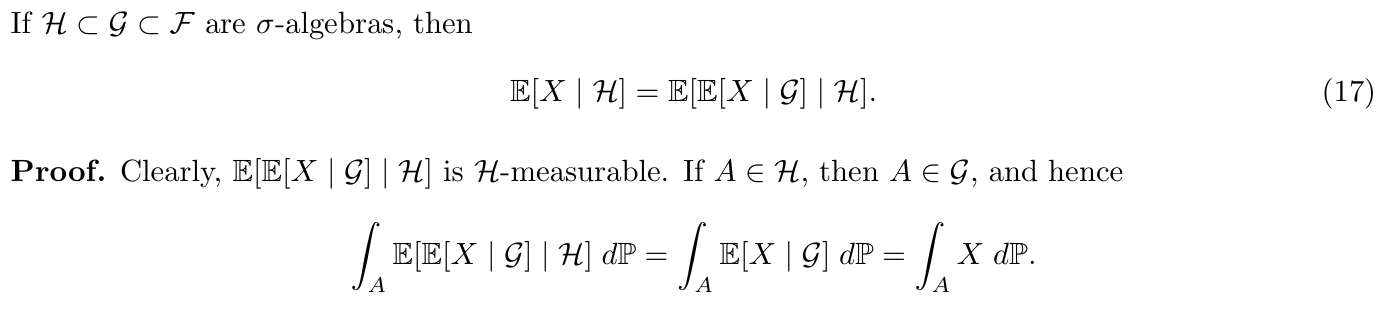
\includegraphics[width=0.5\linewidth]{Images/conditional expectation.png}
    \caption{C.E. Property}
\end{figure}
\[\bbE[X_k \mid X_0 = x] = \bbE[\bbE[X_k \mid X_k] \mid X_0 = x] = \bbE\left[1 + (1 - \frac{2}{N})X_k \mid X_0 = x\right] = 1 + (1-\frac{2}{N})\mu_k\]

    \end{solution}
    \item[(e)] Use the previous part to show that
    \[
    \mu_n = \frac{N}{2} + \left( x - \frac{N}{2} \right) \left( 1 - \frac{2}{N} \right)^n,
    \]
    and hence conclude that \( \mu_n \) converges exponentially rapidly to the equilibrium value of \( \frac{N}{2} \) as \( n \to \infty \).
\begin{solution}
    We induct:
    \begin{enumerate}
        \item For $n = 1,$ we have that 
        \begin{align*}
            \frac{N}{2} + (x- \frac{N}{2})(1 - \frac{2}{N})
            &= \frac{N}{2} + (x - \frac{2}{N}x - \frac{N}{2} + 1)\\
            &= 1 + (1 - \frac{2}{N})x\\
            &= \mu_1.
        \end{align*}
        \item Assume this is true for $n = k$
        \item For $n = k+1,$ we have that by our inductive hypothesis
        \begin{align*}
            \mu_{k+1} &= 1+  (1 - \frac{2}{N})\mu_{k}\\
            &= 1 + (1- \frac{2}{N})\left(\frac{N}{2} + (x - \frac{N}{2})(1 - \frac{2}{N})^k\right)\\
            &= 1 + \frac{N}{2} - 1 + (x- \frac{N}{2})(1-\frac{2}{N})^{k+1}\\
            &= \frac{N}{2} + (x- \frac{N}{2})(1-\frac{2}{N})^{k+1}
        \end{align*}
    \end{enumerate}

Thus, 
\begin{align*}
\mu_n &= \frac{N}{2} + (x - \frac{N}{2})(1- \frac{2}{N})^n\\
&= \frac{N}{2} + (x - \frac{N}{2})\exp\{n \ln(1 - \frac{2}{N}).\} 
\end{align*}
For $N > 2,$ we have that $0 <1- \frac{2}{N}  < 1,$ and thus 
$\ln(1 - \frac{2}{N}) < 0$, and so 
as $n\to \infty,$ $e^{-nc}\to 0,$ and so 
\[\mu_n \to \frac{N}{2}.\]

\end{solution}
\end{enumerate}


\newpage
\section*{Problem 3}
\begin{problem}
A sequence of integers is written on a board starting with the number 12. Each subsequent integer that is written is chosen uniformly randomly from the set of positive divisors of the previous integer (including the possibility of the integer itself). Integers are written until the integer 1 first appears, in which case the process ends. One such sequence is: 12, 6, 6, 3, 3, 3, 1. What is the expected value of the number of terms in the written sequence.
\end{problem}
\begin{solution}
    Define 
    
    \[X_n := \{\text{term on $n$th spot of sequence}\}, \quad
    N_i := \{\text{number of terms in the sequence starting from $i$}\}.\] By assumption, $\bbE[N_1] = 1.$
    
    Then using the law of total expectation: 
\begin{align*}
    \bbE[N_{12}] &= \bbE[\bbE[N_{12} \mid X_1]]\\
    &= 6 + \frac{1}{6}\bbE[N_{12}] + \frac{1}{6}\bbE[N_6] + \frac{1}{6}\bbE[N_4] + \frac{1}{6}\bbE[N_3] + \frac{1}{6}\bbE[N_2] + \frac{1}{6}\bbE[N_1]\\
    &= 6 + \frac{1}{6}\bbE[N_{12}] + \frac{1}{6}\bbE[N_6] + \frac{1}{6}\bbE[N_4] + \frac{1}{6}\bbE[N_3] + \frac{1}{6}\bbE[N_2] + \frac{1}{6}
\end{align*}
We have that 
\[\bbE[N_2] = 1 + \frac{1}{2}\bbE[N_2] + \frac{1}{2}\bbE[N_1] = \frac{3}{2} + \frac{1}{2}\bbE[N_2] \implies \bbE[N_2] = 3\]
For $N_3,$
\begin{align*}
    \bbE[N_3] = 1 + \frac{1}{2}\bbE[N_2] + \frac{1}{2}\bbE[N_1]\\
    &= \frac{3}{2} + \frac{3}{2}\\
    &= 3
\end{align*}
For $N_4$ we have that
\begin{align*}
    \bbE[N_4] &= 1 + \frac{1}{3}\bbE[N_4] + \frac{1}{3}\bbE[N_2] + \frac{1}{3}\bbE[N_1]\\
    &= 1 + \frac{1}{3}\bbE[N_4] + 1 + \frac{1}{3}\\
    &= \frac{7}{3} + \frac{1}{3}\bbE[N_4]\\
    &= \frac{7}{2} = 3.5
\end{align*}
For $N_6$ we have that 
\begin{align*}
    \bbE[N_6] &= 1 + \frac{1}{4}\bbE[N_6] + \frac{1}{4}\bbE[N_3]+ \frac{1}{4}\bbE[N_2] + \frac{1}{4}\bbE[N_1]\\
    &= 1 + \frac{1}{4}\bbE[N_6] + \frac{3}{4} + \frac{3}{4} + \frac{1}{4}\\
    &= \frac{11}{4} + \frac{1}{4}\bbE[N_6]\\
    &= \frac{11}{3}
\end{align*}
Thus, we solve and find that
\[\boxed{\bbE[N_{12}]= \frac{121}{30}}\]

\end{solution}

\newpage
\section*{Problem 4}

Let \( E_k \) be the expected number of flips of a fair coin needed to observe a run of \( k \) heads in a row for the first time.

\begin{enumerate}
    \item[(a)] Explain why \( E_1 = 2 \).
    \begin{solution}
The number of tails before we hit a head if modeled by a geometric variable 
\[Y \sim \text{Geometric}(\frac{1}{2}).\] It is a known fact that if $Y$ is geometric with probability $p,$ then $\bbE[Y] = \frac{1}{p}.$ Thus
        \[E_1 = \bbE[Y] = 2.\]
    \end{solution}
    \item[(b)] Explain why the following recursive equation holds.
    \[
    E_{k+1} = 1 + E_k + \frac{1}{2} E_{k+1}
    \]
\begin{solution}
Suppose we have flipped $k$ heads. It has taken us an expected time of $E_k$ to get here. Thus, our next move is either a tail (in which case it will take us a whole nother $E_{k+1}$ to get to $k+1$ heads again, \textit{plus} the move we just did), or a head, in which case we are done. Thus, we have $\frac{1}{2}(1) + \frac{1}{2}(E_{k+1} + 1) = 1 + \frac{1}{2}E_{k+1}$ as our exhaustive expected value of flips given what will happen in the next move, and obviously need to add the $E_k$ time it took to get here. Thus, in total, 
\[E_{k+1} = 1 + E_k + \frac{1}{2}E_{k+1}\]
\end{solution}
    \item[(c)] Use the recursive relationship from the previous part to find the formula for \( E_k \) for all \( k \).
\begin{solution}
We claim that $E_{k} = 2^{k+1} -2.$
    We have from the above that 
    \[E_{k+1} = 1 + E_k + \frac{1}{2}E_{k+1} \implies E_{k+1} = 2 + 2E_k\] Inducting over $k,$ we see that 
    \begin{enumerate}
        \item For $k = 1,$ we have calculated that $E_1 = 2 = 2^2 -2$ since $E_0$ is clearly $0.$ 
        \item Assume the result holds for $E_n.$ 
        \item For $k = n+1,$ we have that using our inductive hypothesis, 
        \[E_{n+1} = 2 + 2E_{n} = 2 + 2(2^{n+1} -2) = 2 + 2^{n+2} - 4 = 2^{n+2} -2\]
    \end{enumerate}
Note that in order to find the formula, we solved the non-homogeneous equation $E_{k+1} = 2 + 2E_k.$ To do this, we first consider the homogenized version, which is a simple geometric sequence
\[E'_{k} = 2E_{k-1} \implies E'_{k} = E_1\cdot2^{k} = 2^{k+1}.\] Then we add it back into the non-homogeneous sequence by assuming that $E''_{k} = a$ for any $k.$ Then 
\[a = 2 + 2a \implies a = -2.\] Then we solve by 
\[E_k = E_k' + E_k'' = 2^{k+1} - 2\]
\end{solution}
\end{enumerate}

\newpage
\section*{Problem 5}
\begin{problem}
    
Recall a stochastic matrix is one in which the row sums all equal 1. We call a stochastic matrix \textit{doubly stochastic} if the columns add up to 1 as well. Suppose \( P \) is the transition matrix for an irreducible, aperiodic Markov chain and that \( P \) is doubly stochastic.
\end{problem}

\begin{enumerate}
    \item[(a)] Show that the invariant distribution is uniform.
\begin{solution}
    First, since $\{X_n\}$ is irreducible and aperiodic, then there is exists some unique $\pi$ stationary distribution. Thus, it suffices to find a solution satisfying 
    \begin{align}
        \pi P = \pi
    \end{align} and that will prove to be the only solution. We offer the candidate solution of 
    \[\pi_0 = \pi_1 = \dots = \pi_N.\]
    Since $P$ is doubly stochastic, we have that for any column $0\leq k\leq N$
\[\sum_{n=0}^N \pi_n p(n,k) = \sum_{n=0}^N \pi_0p(n,k)= \pi_0\sum_{n=0}^N p(n,k) = \pi_0 = \pi_k.\] Thus, this candidate $\pi$ satisfies (1). Thus, the requirement that $\pi$ is a probability vector forces 
\[\sum_{n=0}^N \pi_n = n\pi_0 = 1,\] and thus 
\[\pi = \begin{pmatrix}
    \frac{1}{N} & \frac{1}{N} & \cdots & \frac{1}{N}
\end{pmatrix}\]
\end{solution}
    \item[(b)] Consider the following Markov chain on shuffles, that is, on orderings of a standard 52-card deck of cards where the transitions are: at each time a random card is chosen from the deck (with all 52 cards equally likely to be chosen) and is put on the top of the deck.
    \begin{enumerate}
        \item[(i)] Show that this is irreducible, aperiodic, and has a doubly stochastic transition matrix.
    \begin{solution}
        The state space is the 
        \[S = \sigma\{1,2,3,\dots, 51,52\},\] where $\sigma$ represents all the possible permutations of $\{1,2,3,\dots, 52\}$ Then $P \in \mathcal{M}_{52! \times 52!}.$ If $n \in S,$ then since there is a $\frac{1}{52}$ chance of choosing the top card (the only card in which the ordering won't be impacted), then $p(n,n) = \frac{1}{52}.$ Thus the Markov chain is aperiodic. 
        Suppose $X_0 = i.$ Then $X_1 = j,$ where $j$ is a permutation of $i$ with exactly one number different.  Clearly, $p(i,j) = \frac{1}{52}.$  We claim that there are $51$ permutations that differ by one move. To see this, it suffices to show that 
        $\{1,2,3,\dots, 52\}$ has $52$ moves. It has the trivial move, that is, the one where $1$ is chosen. Then there is 
        \[\sigma_1\{1,2,3\dots, 52\} = \begin{cases}
            \{1,2,3\dots, 52\}\\
            \{2,1, 3\dots, 52\}\\
            \{3,1,2\dots, 52\}\\
            \vdots\\
            \{52,1,2\dots, 52\}
        \end{cases}.\] There is nothing special about the permutation that we chose, so then each permutation can go to $52$ others with uniform probability of $\frac{1}{52}.$ Thus, each permutation can come from exactly $52$ different permutations This shows that $\{X_n\}$ is a doubly stochastic matrix since 
        \[\sum_{n=1}^{52!}p(n, 1) = \sum_{\text{permutations that go to $\{1,2,3,\dots, 52\}$}}\frac{1}{52} = 52\cdot 52 = 1.\]

        It remains to see that $\{X_n\}$ is irreducible.  If $i,j \in S$ differ from each other by $n$ spots. Let $I = \{i_1, \dots, i_n\}$ be the spots the permutation differ. We will show that we can permute $i\to j.$ There is a $\frac{1}{52}$ chance the $i_n$ spot is chosen from $i$. Note that the card on this spot in $j$ will necessarily be before $i_n.$ Thus, we have a $\frac{1}{52}$ chance of choosing the card at this spot until both cards are the same. Thus, 
        \[\bbP\{I = \{i_1, \dots, i_{n-1}\}\} >\frac{1}{52^{52 - i_n}}\] One can keep going like this to show that $\bbP\{I = \emptyset\} >0.$ Thus, we have showed that $i \to j.$ But there was nothing special about starting with $i.$ In fact, because $I = J,$ where $J$ is the spots where $j$ differs from $i,$ then 
        \[\bbP\{J = \emptyset\} = \bbP\{I = \emptyset\} >0.\] Thus, $j\to i.$
    \end{solution}
        \item[(ii)] Suppose we start the chain with a perfectly ordered deck and we do this “shuffle” until the deck returns to being perfectly ordered. If we make one move every second, what is the expected number of years until this happens?
    \begin{solution}
        Let $\sigma_1  = \{1,2,3,\dots, 52\}.$ Define
        \[T_{\sigma_1} = \{n >0 \mid X_n = \sigma_1\}.\] From the previous problem and part (a), we know that 
        \[\pi_{\sigma_i} = \frac{1}{52!}, \quad \sigma_i \in \sigma\{1,2,3,\dots, 52\}.\] Thus, 
        \[\bbE[T_{\sigma_1}] = \frac{1}{\pi_{\sigma_1}} = 52!.\] Thus, it will take
        \[52! \text{ sec} \cdot \frac{1\text{ min}}{60 \text{ sec}}\cdot \frac{1 \text{ hr}}{60\text{ min}}\cdot \frac{1 \text{ day}}{24 \text{hr}}\cdot \frac{1 \text{ year}}{365 \text{ days}}\approx \boxed{2.558 \times 10^{60}\text{ years}}\]
    \end{solution}
    \end{enumerate}
\end{enumerate}

\newpage
\section*{Problem 6}
\begin{problem}
 Let \(\{X_n\}\) be a Markov chain on a countable space \(S\), with transition probabilities \(p(x,y)\). A function \(\pi : S \to [0,1]\) with \(\sum_{x \in S} \pi_x = 1\) is called a reversible distribution for \(\{X_n\}\) if:
\[
\pi_x p(x,y) = \pi_y p(y,x), \quad \forall x, y \in S.
\]

\begin{enumerate}
    \item[(a)] Show that a reversible distribution is also a stationary distribution.
\begin{solution}
    First off, if $\pi$ is a reversible distribution then it is a valid probability distribution since $\sum_{x\in S}\pi_x = s.$ First note that since the transition probabilities add up to $1$ for each 'row,' we have that for any $k \in \bbN,$ 
    \[\sum_{n=1}^\infty \pi_n p(n,k)= \sum_{n=1}^\infty \pi_k p(k,n) = \pi_k \sum_{n=1}^\infty p(k,n) = \pi_k.\] Thus, if $P$ is the countably infinite transition matrix, we have that $\pi P  = \pi.$ 
\end{solution}
    \item[(b)] Give an example of a Markov chain \(\{X_n\}\) and a stationary distribution for \(\{X_n\}\) which is not reversible.
\begin{solution}
    Consider a Markov chain $\{X_n\}$ in $S = \{1,2,3\}.$ Then if 
    \[P = \begin{pmatrix}
        0 & 1 & 0 \\
        0 & 0 & 1\\
        1 & 0 & 0
    \end{pmatrix},\] it is not hard to show that 
    \[\pi = \begin{pmatrix}
        \frac{1}{3}\\
        \frac{1}{3}\\
        \frac{1}{3}
    \end{pmatrix}.\] However, we have that 
    \[\pi_1 p(1,3) = 0\neq \pi_3p(3,1) =\frac{1}{3}.\] Thus $\{X_n\}$ is not reversible. 
\end{solution}
    \item[(c)] Show that if \(\pi\) is a reversible distribution and \(X_0\) has the distribution \(\pi\) (i.e., \(P[X_0 = x] = \pi_x\) for each \(x \in S\)), then for any \(n\), \((X_n, X_{n-1}, \ldots, X_0)\) has the same distribution as \((X_0, X_1, \ldots, X_n)\). 
    \begin{itemize}
        \item[\textbf{Hint:}] Consider states \(x_0, \ldots, x_n \in S\) and show that:
        \[
        P[X_0 = x_0, X_1 = x_1, \ldots, X_n = x_n] = P[X_n = x_0, X_{n-1} = x_1, \ldots, X_0 = x_n].
        \]
    \end{itemize}
    \begin{solution}
    We assume, as always, that $\{X_n\}$ is a time homogeneous process. 
        Let $x_0, \dots, x_n \in S.$ We claim that the distribution of $\{X_n\}$ starting at $x_0$ and ending at $x_n$ is the same as if it started at $x_n$ and ended at $x_0.$ 
        \[\bbP\{X_0 = x_0, X_1 = x_1, \ldots, X_n = x_n\}\] To see this, consider that by the Markov property and Bayes' rule and finally the time-homogeneity, (and the redoing all of that)
        \begin{align*}
            \bbP\{X_n = x_n, \dots,X_0 = x_0\} &= \bbP\{X_n  = x_n \mid X_{n-1}  = x_{n-1}, \dots, X_0 = x_0\} \bbP\{X_{n-1}  = x_{n-1}, \dots, X_0 = x_0\}\\
            &= \bbP\{X_n = x_n \mid X_{n-1} = x_{n-1}\}\bbP\{X_{n-1}  = x_{n-1}, \dots, X_0 = x_0\}\\
            &= \dots\\
            &= \bbP\{X_n = x_n \mid X_{n-1} = x_{n-1}\}\bbP\{X_{n-1} = x_{n-1}\mid X_{n-2} = x_{n-2}\}\cdots \bbP\{X_1 = x_1 \mid X_0 = x_0\}\bbP\{X_0 = x_0\}\\
            &= p(x_{n-1}, x_n)p(x_{n-2}, x_{n-1})\cdots p(x_0, x_1)\bbP\{X_0 = x_0\}\\
            &= \pi_{x_0} p(x_0, x_1)\cdots p(x_{n-1}, x_{n-2})p(x_{n-1},x_n)\\
            &= \pi_{x_1}p(x_1, x_0) p(x_1, x_2)\cdots p(x_{n-1}, x_{n-2})p(x_{n-1},x_n)\\
            &= p(x_1, x_0)\pi_{x_2}p(x_2, x_1)\cdots p(x_{n-1}, x_{n-2})p(x_{n-1},x_n)\\
            &= \dots\\
            &= p(x_1, x_0)p(x_2, x_1)\cdots p(x_{n-2}, x_{n-1})\pi_{n-1}p(x_{n-1},x_n)\\
            &= p(x_1, x_0)p(x_2, x_1)\cdots p(x_{n-2}, x_{n-1})p(x_n, x_{n-1})\pi_{x_n}\\
            &= \bbP\{X_0 = x_n\}\bbP\{X_1 = x_{n-1} \mid X_0 = x_{n}\}\cdots \bbP\{X_n = x_0 \mid X_{n-1} = x_1\}\\
            &= \bbP\{X_0 = x_n, X_1 = x_{n-1}, \dots, X_n = x_0\}
        \end{align*}
    \end{solution}
\end{enumerate}
\end{problem}


\end{document}

